After performing the simulations we can now gather the results. The simulations are done in two steps. First, 2,500,000 iterations are used to find equilibrium, where both $\beta$ and the step size are continuously updated as explained above. After equilibrium has been reached, 10,000,000 iterations are used to calculate the energy. This process is repeated for 50 values of the separation s between 1 and 2 a.u. This gives the following result:
\begin{figure}[H]
	\centering
	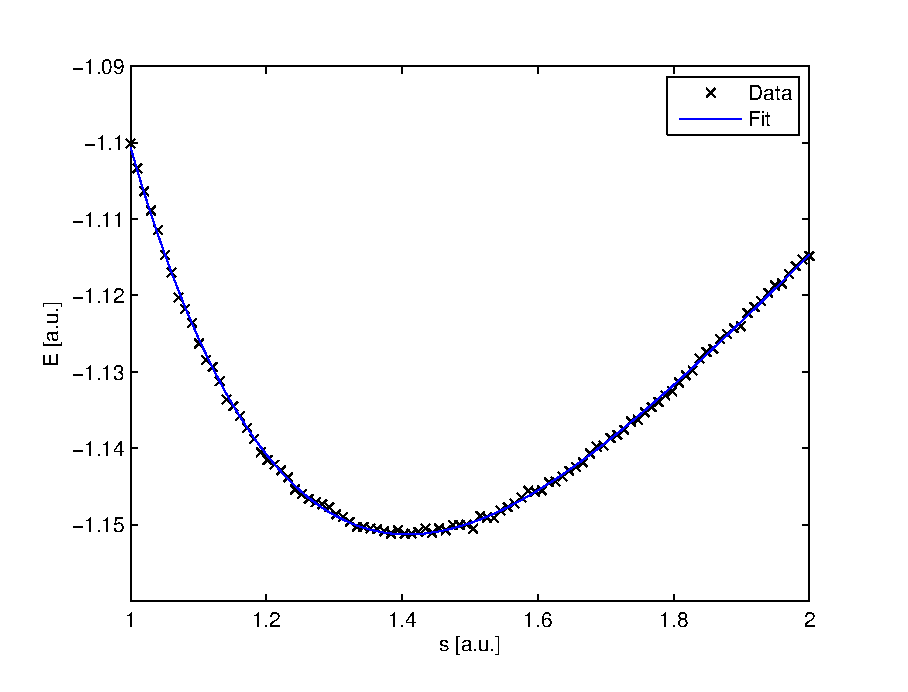
\includegraphics[width=0.8\textwidth]{plot.eps}
	\caption{The total energy of the hydrogen molecule calculated using Variational Monte Carlo (black crosses). The blue fitted line is the Morse potential, given in Equation~\ref{eq:Morse}.}
	\label{plot}
\end{figure}
\newpage
\noindent  In this plot, the data points calculated by the simulation are shown. We have also fitted these data points with a so-called Morse potential. This potential is given by
\begin{align}
V = D{\left( {1 - {e^{ - a\left( {s - {s_0}} \right)}}} \right)^2} - {V_0}.
\label{eq:Morse}
\end{align}
In this expression, $D$ is the dissociation energy, $s_0$ is the equilibrium separation, $V_0$ is the equilibrium energy and $a$ is given by
\begin{align}
a = \sqrt{\frac{K}{2D}},
\end{align}
with K the spring constant of the potential. At this point, it is good to note that there are two ways to find the dissociation energy D. One can find it directly through the fit parameters, or one can use:
\begin{align}
D = {V_0} - 1.
\end{align}
In this report, we use the expression above to find D. The reason for this is that both the parameters $a$ and $D$ have a similar effect on the form of the potential. Therefore, when only examining a small part of the total potential, these parameters can be rather uncertain. $V_0$, on the other hand, fits the lowest part of the curve (the part we are most interested in) much better, as it does not care for the rest of the curve. Therefore, we use $V_0$ to find a value for the dissociation energy.\\
The spectrum of the Morse potential can be calculated analytically. This gives~\cite{jose_pdf}:
\begin{align}
{E_n} = \hbar \omega \left( {n + \frac{1}{2}} \right)\left( {1 - \frac{{\hbar \omega \left( {n + \frac{1}{2}} \right)}}{{4D}}} \right),
\end{align}
with $\omega=\sqrt{\frac{K}{M}}$, where M is the reduced mass of the hydrogen molecule. In atomic units, we can write\newline M = 925.260 a.u.\cite{hyplink}. By fitting the data points we have found, we can now find values for these parameters and compare the results:
\begin{table}[H]
\centering
\begin{tabular}{|l|l|}
\hline
\textit{Parameter} & \textit{Result {[}a.u.{]}} \\ \hline
\textbf{Results}   &                            \\\hline
$D$                  & 0.1512 $\pm$ 0.0001              \\\hline
$R_0$                 & 1.408  $\pm$0.002              \\\hline
$\hbar\omega$               & 0.02037 $\pm$0.00007                            \\\hline
\textbf{Results simulation Jose}                   &                            \\\hline
$D$                   &       0.15123(3)                     \\\hline
$R_0$                   &           1.4054(2)                 \\\hline
 $\hbar\omega$                  &      0.02044(2)                      \\\hline
 \textbf{Literature}                  &                            \\\hline
  $D$                 &   0.1645(6)                         \\\hline
    $R_0$               &      1.40111(9)                      \\\hline
     $\hbar\omega$               &     0.02005(3)          \\          
     \hline
\end{tabular}
\caption{Values for the parameters $D$, $R_0$ and $\hbar\omega$ found with fitting our data points, from the simulation performed by Jose~\cite{jose_pdf} and literature ($D$ taken from~\cite{traynor1991}, $R_0$ and $\hbar\omega$ from~\cite{jose_pdf}).}
\end{table}
\newpage
\subsection{Discussion}
Comparing our results with the results of a similar simulation by Jose and with the literature, we see that our results are quite comparable to the results obtained by Jose, but we also see that the literature values are somewhat different. 

The fact that our results are very similar to those found by Jose makes a lot of sense, as our approach is almost exactly the same. The good agreement does indicate that our simulation is working as intended, however, so it is still useful to do this comparison. One difference between the two approaches is the number of walkers used. We used fewer walkers than Jose, meaning that we needed more iterations to find the results. 

The agreement of our results with values found in literature is less good, however. The separation distance and oscillation frequency are quite reasonable, but the dissociation energy is rather low. The most probable explanation for this is that there are extra effects that we have not taken into account. This would mean that our trial wave function is not as good as we think it is, leading to a less tight lower bound for the dissociation energy. It is good to note that the fact that our value of the dissociation energy is lower at least indicates that our approach is valid, as we are looking for a lower bound for the dissociation energy (since the total energy is negative, an upper bound for the energy corresponds to a lower bound for the dissociation energy).

A couple of things could be done in order to improve our simulation. First of all, more iterations could be used to calculate the energy. More iterations could be used per point to reduce the uncertainty per point, and more values of the separation distance could be used to increase the accuracy of the fit. Alternatively, more walkers could be used. This has a very similar effect to using more iterations, and would improve the result in a similar way.

More drastically, one could try to find a better trial wave function for the hydrogen molecule. As discussed above, the upper bound found for the energy is not particularly impressive for variational calculus. Therefore, finding a better trial wave function may yield a tighter upper bound, improving the results of the simulation. However, finding a good trial wave function can be rather difficult, making this a rather drastic option. 

